\newcommand{\dissectionTikz}[2]{ % args = number vertices, list edges i/j
	\begin{tikzpicture}[scale=.4]
		\foreach \i in {1,...,#1} {
			\node[draw, circle, fill, inner sep=.5pt] (v\i) at (90+360/#1*\i-180/#1:1) {}; % vertices of polygon
			\draw[-] (90+360/#1*\i-180/#1:1) -- (90+360/#1*\i+180/#1:1); % boundary edges of polygon
		};
		\foreach \i/\j in {#2} {
			\draw[-] (v\i) -- (v\j); % draw the edges
		};
	\end{tikzpicture}
}
\newcommand{\whiteDissectionTikz}[2]{ % args = number vertices, list edges i/j
	\begin{tikzpicture}[baseline=-3pt,scale=.4]
		\foreach \i in {1,...,#1} {
			\node[draw, circle, fill, inner sep=.75pt, outer sep=0pt] (v\i) at (90+360/#1*\i-360/#1:1) {}; % vertices of polygon
			\draw[-, line width=1.25pt] (90+360/#1*\i-360/#1:1) -- (90+360/#1*\i:1); % boundary edges of polygon
		};
		\foreach \i/\j in {#2} {
			\draw[-, line width=1.25pt] (v\i) -- (v\j); % draw the edges
		};
		\foreach \i in {1,...,#1} {
			\node[draw, circle, fill, inner sep=.5pt, outer sep=0pt, white] (v\i) at (90+360/#1*\i-360/#1:1) {}; % vertices of polygon
			\draw[-,white] (90+360/#1*\i-360/#1:1) -- (90+360/#1*\i:1); % boundary edges of polygon
		};
		\foreach \i/\j in {#2} {
			\draw[-,white] (v\i) -- (v\j); % draw the edges
		};
	\end{tikzpicture}
}

\newcommand{\projModule}[1]{
	\begin{tikzpicture}[scale=.3]
		\foreach \q [count=\i] in {#1} {
        	\let\mymatrixcontent\empty
        	\foreach \c in \q {%
            	\expandafter\gappto\expandafter\mymatrixcontent\expandafter{\c\\[-.1cm]}%
        	    % or
            	%\xappto\mymatrixcontent{\expandonce{\c\\}}
    	    }
	    	\ifthenelse{\i>1}{\node (m\i) at (2*\i-1,0) {$\oplus$};}{}
    		\node (m\i) at (2*\i,0) {$\begin{matrix} \mymatrixcontent \end{matrix}$};
		}
	\end{tikzpicture}
}

\newcommand{\hgap}{1.5}
\newcommand{\vgap}{2.5}
\newcommand{\associahedronAccordionTikz}{
	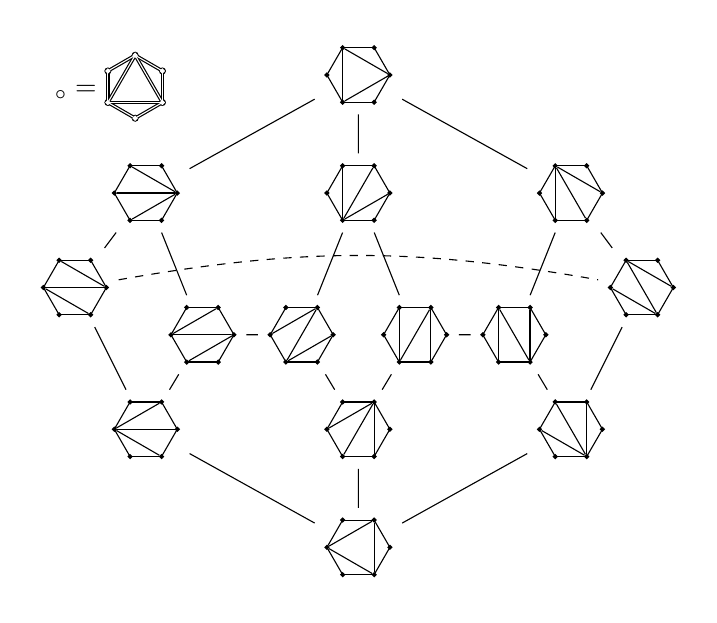
\begin{tikzpicture}[scale=.6]
	\useasboundingbox (-1,-1) rectangle(8*\hgap+1, 4*\vgap+1);
		% vertices = triangulations
    	\node (t1)  at (  4*\hgap,   4*\vgap) {\dissectionTikz{6}{1/3, 1/5, 3/5}};
    	\node (t2)  at (  1*\hgap,   3*\vgap) {\dissectionTikz{6}{1/5, 2/5, 3/5}};
    	\node (t3)  at (  4*\hgap,   3*\vgap) {\dissectionTikz{6}{1/3, 3/5, 3/6}};
    	\node (t4)  at (  7*\hgap,   3*\vgap) {\dissectionTikz{6}{1/3, 1/4, 1/5}};
    	\node (t5)  at (  0*\hgap, 2.2*\vgap) {\dissectionTikz{6}{1/5, 2/5, 2/4}};
    	\node (t6)  at (  8*\hgap, 2.2*\vgap) {\dissectionTikz{6}{1/5, 1/4, 2/4}};
    	\node (t7)  at (1.8*\hgap, 1.8*\vgap) {\dissectionTikz{6}{2/6, 2/5, 3/5}};
    	\node (t8)  at (3.2*\hgap, 1.8*\vgap) {\dissectionTikz{6}{2/6, 3/6, 3/5}};
    	\node (t9)  at (4.8*\hgap, 1.8*\vgap) {\dissectionTikz{6}{1/3, 3/6, 4/6}};
    	\node (t10) at (6.2*\hgap, 1.8*\vgap) {\dissectionTikz{6}{1/3, 1/4, 4/6}};
	  	\node (t11) at (  1*\hgap,   1*\vgap) {\dissectionTikz{6}{2/6, 2/5, 2/4}};
    	\node (t12) at (  4*\hgap,   1*\vgap) {\dissectionTikz{6}{2/6, 3/6, 4/6}};
    	\node (t13) at (  7*\hgap,   1*\vgap) {\dissectionTikz{6}{1/4, 2/4, 4/6}};
    	\node (t14) at (  4*\hgap,   0*\vgap) {\dissectionTikz{6}{2/6, 2/4, 4/6}};
		% edges = flips
		\draw[-] (t1) -- (t2);
		\draw[-] (t1) -- (t3);
		\draw[-] (t1) -- (t4);
		\draw[-] (t2) -- (t5);
		\draw[-] (t2) -- (t7);
		\draw[-] (t3) -- (t8);
		\draw[-] (t3) -- (t9);
		\draw[-] (t4) -- (t10);
		\draw[-] (t4) -- (t6);
		\draw[-, dashed] (t5) edge[bend left=10] (t6);
		\draw[-] (t5) -- (t11);
		\draw[-] (t6) -- (t13);
		\draw[-] (t7) -- (t8);
		\draw[-] (t7) -- (t11);
		\draw[-] (t8) -- (t12);
		\draw[-] (t9) -- (t10);
		\draw[-] (t9) -- (t12);
		\draw[-] (t10) -- (t13);
		\draw[-] (t11) -- (t14);
		\draw[-] (t12) -- (t14);
		\draw[-] (t13) -- (t14);

    \node (reference) at (0.5*\hgap, 6.5*\hgap) {$\dissection_\circ = \whiteDissectionTikz{6}{1/3, 1/5, 3/5}$};
	\end{tikzpicture}
}

\newcommand{\associahedronSiltingTikz}{
	\begin{tikzpicture}[scale=.6, vert/.style={inner sep=1pt}]
	\useasboundingbox (-1,-1) rectangle(8*\hgap+1, 4*\vgap+1);
		% vertices = triangulations
    	\node[vert] (t1)  at (  4*\hgap,   4*\vgap) {\projModule{{2,1}, {3,2}, {1,3}}};
    	\node[vert] (t2)  at (  1*\hgap,   3*\vgap) {\projModule{{3}, {3,2}, {1,3}}};
    	\node[vert] (t3)  at (  4*\hgap,   3*\vgap) {\projModule{{2,1}, {1}, {1,3}}};
    	\node[vert] (t4)  at (  7*\hgap,   3*\vgap) {\projModule{{2,1}, {3,2}, {2}}};
    	\node[vert] (t5)  at (  0*\hgap, 2.2*\vgap) {\projModule{{3}, {3,2}}};
    	\node[vert] (t6)  at (  8*\hgap, 2.2*\vgap) {\projModule{{3,2}, {2}}};
    	\node[vert] (t7)  at (1.8*\hgap, 1.8*\vgap) {\projModule{{3}, {1,3}}};
    	\node[vert] (t8)  at (3.2*\hgap, 1.8*\vgap) {\projModule{{1}, {1,3}}};
    	\node[vert] (t9)  at (4.8*\hgap, 1.8*\vgap) {\projModule{{2,1}, {1}}};
    	\node[vert] (t10) at (6.2*\hgap, 1.8*\vgap) {\projModule{{2,1}, {2}}};
    	\node[vert, inner sep=2pt] (t11) at (  1*\hgap,   1*\vgap) {\projModule{{3}}};
    	\node[vert, inner sep=2pt] (t12) at (  4*\hgap,   1*\vgap) {\projModule{{1}}};
    	\node[vert, inner sep=2pt] (t13) at (  7*\hgap,   1*\vgap) {\projModule{{2}}};
    	\node[vert, inner sep=4pt] (t14) at (  4*\hgap,   0*\vgap) {$\varnothing$};
		% edges = flips
		\draw[-] (t1) -- (t2);
		\draw[-] (t1) -- (t3);
		\draw[-] (t1) -- (t4);
		\draw[-] (t2) -- (t5);
		\draw[-] (t2) -- (t7);
		\draw[-] (t3) -- (t8);
		\draw[-] (t3) -- (t9);
		\draw[-] (t4) -- (t10);
		\draw[-] (t4) -- (t6);
		\draw[-, dashed] (t5) edge[bend left=10] (t6);
		\draw[-] (t5) -- (t11);
		\draw[-] (t6) -- (t13);
		\draw[-] (t7) -- (t8);
		\draw[-] (t7) -- (t11);
		\draw[-] (t8) -- (t12);
		\draw[-] (t9) -- (t10);
		\draw[-] (t9) -- (t12);
		\draw[-] (t10) -- (t13);
		\draw[-] (t11) -- (t14);
		\draw[-] (t12) -- (t14);
		\draw[-] (t13) -- (t14);

    \node (reference) at (0.5*\hgap, 6.5*\hgap) {
      $\overline{\quiver} = \begin{tikzpicture}[baseline=-3pt,scale=0.4,decoration={markings, mark=at position 0.6 with {\arrow{angle 90}}} ]
        \node (n1) at (150:1.5) {1};
        \node (n2) at (30:1.5) {2};
        \node (n3) at (270:1.5) {3};
        \draw[-, postaction=decorate] (n1) -- (n2);
        \draw[-, postaction=decorate] (n2) -- (n3);
        \draw[-, postaction=decorate] (n3) -- (n1);
        \draw[-] ([shift={(30:1.5)}]180:0.8) arc (180:240:0.8);
        \draw[-] ([shift={(150:1.5)}]0:0.8) arc (360:300:0.8);
        \draw[-] ([shift={(270:1.5)}]60:0.8) arc (60:120:0.8);
      \end{tikzpicture}$
    };
	\end{tikzpicture}
}

\newcommand{\accordiohedronAccordionTikz}{
	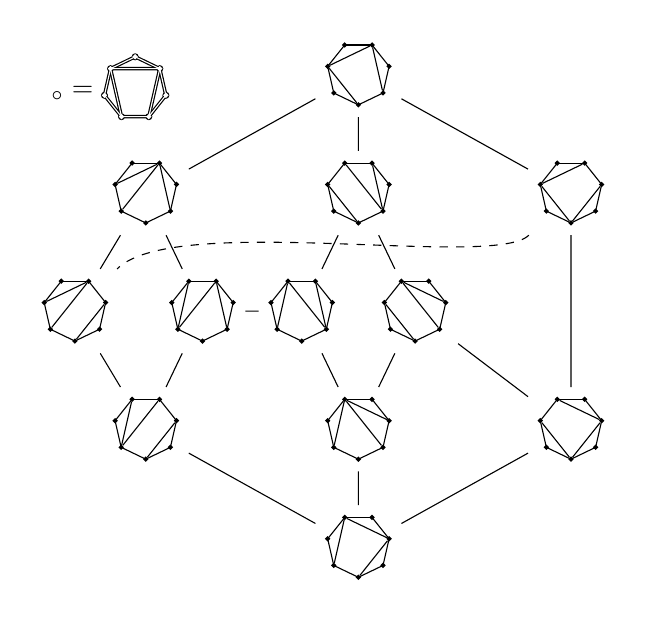
\begin{tikzpicture}[scale=.6]
	\useasboundingbox (-1,-1) rectangle(7*\hgap+1, 4*\vgap+1);
		% vertices = triangulations
    	\node (t1)  at (  4*\hgap, 4*\vgap) {\dissectionTikz{7}{2/4, 2/7, 5/7}};
    	\node (t2)  at (  1*\hgap, 3*\vgap) {\dissectionTikz{7}{2/7, 3/7, 5/7}};
    	\node (t3)  at (  4*\hgap, 3*\vgap) {\dissectionTikz{7}{5/7, 1/5, 2/4}};
    	\node (t4)  at (  7*\hgap, 3*\vgap) {\dissectionTikz{7}{2/4, 2/7, 4/6}};
    	\node (t5)  at (  0*\hgap, 2*\vgap) {\dissectionTikz{7}{2/7, 3/7, 4/6}};
    	\node (t7)  at (1.8*\hgap, 2*\vgap) {\dissectionTikz{7}{1/3, 3/7, 5/7}};
    	\node (t8)  at (3.2*\hgap, 2*\vgap) {\dissectionTikz{7}{1/3, 1/5, 5/7}};
    	\node (t9)  at (4.8*\hgap, 2*\vgap) {\dissectionTikz{7}{1/5, 1/6, 2/4}};
    	\node (t11) at (  1*\hgap, 1*\vgap) {\dissectionTikz{7}{1/3, 3/7, 4/6}};
    	\node (t12) at (  4*\hgap, 1*\vgap) {\dissectionTikz{7}{1/3, 1/5, 1/6}};
    	\node (t13) at (  7*\hgap, 1*\vgap) {\dissectionTikz{7}{1/6, 2/4, 4/6}};
    	\node (t14) at (  4*\hgap, 0*\vgap) {\dissectionTikz{7}{1/3, 1/6, 4/6}};
		% edges = flips
		\draw[-] (t1) -- (t2);
		\draw[-] (t1) -- (t3);
		\draw[-] (t1) -- (t4);
		\draw[-] (t2) -- (t5);
		\draw[-] (t2) -- (t7);
		\draw[-] (t3) -- (t8);
		\draw[-] (t3) -- (t9);
		\draw[-, dashed] (t4) to[in=45, in looseness=.5, out=-135, out looseness=.3] (t5);
		\draw[-] (t4) -- (t13);
		\draw[-] (t5) -- (t11);
		\draw[-] (t7) -- (t8);
		\draw[-] (t7) -- (t11);
		\draw[-] (t8) -- (t12);
		\draw[-] (t9) -- (t12);
		\draw[-] (t9) -- (t13);
		\draw[-] (t11) -- (t14);
		\draw[-] (t12) -- (t14);
		\draw[-] (t13) -- (t14);

    \node (reference) at (0.5*\hgap, 6.5*\hgap) {$\dissection_\circ = \whiteDissectionTikz{7}{2/4, 2/7, 5/7}$};
	\end{tikzpicture}
}

\newcommand{\accordiohedronSiltingTikz}{
	\begin{tikzpicture}[scale=.6, vert/.style={inner sep=1pt}]
	\useasboundingbox (-1,-1) rectangle(7*\hgap+1, 4*\vgap+1);
		% vertices = triangulations
    	\node[vert] (t1)  at (  4*\hgap, 4*\vgap) {\projModule{{1}, {2,1}, {3,2}}};
    	\node[vert] (t2)  at (  1*\hgap, 3*\vgap) {\projModule{{2}, {2,1}, {3,2}}};
    	\node[vert] (t3)  at (  4*\hgap, 3*\vgap) {\projModule{{1}, {3,2}, {3}}};
    	\node[vert] (t4)  at (  7*\hgap, 3*\vgap) {\projModule{{1}, {2,1}}};
    	\node[vert] (t5)  at (  0*\hgap, 2*\vgap) {\projModule{{2}, {2,1}}};
    	\node[vert] (t7)  at (1.8*\hgap, 2*\vgap) {\projModule{{2}, {3,2}}};
    	\node[vert] (t8)  at (3.2*\hgap, 2*\vgap) {\projModule{{3}, {3,2}}};
    	\node[vert] (t9)  at (4.8*\hgap, 2*\vgap) {\projModule{{1}, {3}}};
    	\node[vert, inner sep=2pt] (t11) at (  1*\hgap, 1*\vgap) {\projModule{{2}}};
    	\node[vert, inner sep=2pt] (t12) at (  4*\hgap, 1*\vgap) {\projModule{{3}}};
    	\node[vert, inner sep=2pt] (t13) at (  7*\hgap, 1*\vgap) {\projModule{{1}}};
    	\node[vert, inner sep=4pt] (t14) at (  4*\hgap, 0*\vgap) {$\varnothing$};
		% edges = flips
		\draw[-] (t1) -- (t2);
		\draw[-] (t1) -- (t3);
		\draw[-] (t1) -- (t4);
		\draw[-] (t2) -- (t5);
		\draw[-] (t2) -- (t7);
		\draw[-] (t3) -- (t8);
		\draw[-] (t3) -- (t9);
		\draw[-, dashed] (t4) to[in=45, in looseness=.5, out=-135, out looseness=.3] (t5);
		\draw[-] (t4) -- (t13);
		\draw[-] (t5) -- (t11);
		\draw[-] (t7) -- (t8);
		\draw[-] (t7) -- (t11);
		\draw[-] (t8) -- (t12);
		\draw[-] (t9) -- (t12);
		\draw[-] (t9) -- (t13);
		\draw[-] (t11) -- (t14);
		\draw[-] (t12) -- (t14);
		\draw[-] (t13) -- (t14);

    \node (reference) at (0.5*\hgap, 6.5*\hgap) {
      $\overline{\quiver}(\dissection_\circ) = \begin{tikzpicture}[baseline=-3pt,scale=0.4,decoration={markings, mark=at position 0.6 with {\arrow{angle 90}}} ]
        \node (n1) at (0,0) {1};
        \node (n2) at (2,0) {2};
        \node (n3) at (4,0) {3};
        \draw[-, postaction=decorate] (n1) -- (n2);
        \draw[-, postaction=decorate] (n2) -- (n3);
        \draw[-] ([shift={(2.7,0)}]0:0) arc (0:180:0.7);
      \end{tikzpicture}$
    };
	\end{tikzpicture}
}
